%%
%% This is file `example-1.tex',
%% generated with the docstrip utility.
%%
%% The original source files were:
%%
%% drexel-thesis.dtx  (with options: `example-part')
%% 
%% This is a generated file.
%% 
%% Copyright (C) 2010 W. Trevor King
%% 
%% This file may be distributed and/or modified under the conditions of
%% the LaTeX Project Public License, either version 1.3 of this license
%% or (at your option) any later version.  The latest version of this
%% license is in:
%% 
%%    http://www.latex-project.org/lppl.txt
%% 
%% and version 1.3 or later is part of all distributions of LaTeX version
%% 2003/06/01 or later.
%% 

\chapter{Quasi 2-D and 2.5-D Systems}
Studies of traveling waves have focused on two-dimensional waves that spread parallel to the surface (pia) of the brain \citep{reimer2010}\citep{keane2015}\citep{Townsend2018}\citep{Golomb1997}\citep{Qi2015}. 
This is to be expected as this is the geometry of the system on which they are observed, and \citep{Wilson1973} provide an anatomical argument for focusing on such structure. 

We now extend our study of traveling waves in quasi 1-D minicolumns to two-dimensional topologies.
First we study two-dimensional sheets of neurons extended in the X and Y directions.
As before, we find that our model doesn't support traveling waves in a purely two-dimensional sheet (Z=1) under the model parameters studied.
When we extend the system to a quasi two-dimensional sheet (Z=2) we find traveling waves are evoked by both the background and impulsive stimulus.

We then further extend our topology to what we term a ``forest'' of minicolumns.
This structure consists of an ensemble of our minicolumns arranged on a grid, with the Z extent less than the X/Y extents.
We find that our forest supports trasverse traveling waves in the X/Y plane.

\section{Two-dimensional sheets of neurons}
Traveling waves in two-dimensional neuronal sheets have been studied in the brain \citep{huang2004}\citep{Townsend2018} and in simulation\citep{keane2015}\citep{Spreizer2019}
While one-dimensional waves have only one structure, the additional degree of freedom in two dimensions allows for several categories of waves.
These include circular waves that spread outward from a point, large plane waves that propagate over the entire surface and spiral waves\citep{Huang2010} that rotate around a phase singularity.
Different types of waves have been associated with different elements of visual stimulus\citep{Benucci2007}.
We find evidence for all these categories of waves in our quasi two-dimensional sheet.

Each sheet consists of neurons placed on a unit grid. 
The X and Y extents are much larger than the Z extent.
We generally use sheets with Z=2 with the exception of one purely two-dimensional example with Z=1.
Neurons are created and connected as described in Methods.
Due to the larger area of regard and the more demanding computational experiments we use periodic boundary conditions in our quasi two-dimensional sheets.
A small example quasi 2-D sheet is shown in Figure \ref{fig:sheet_structure}.
In this small example the periodic boundary conditions are easily seen in the connection matrix.

\begin{figure}[!htb]
 \caption{Example small quasi 2-D sheet with dimensions X=20, Y=20, Z=2, $\lambda$=2.5, and C=0.5. 
 a)  Sheet showing connections between neurons as lines colored using a color scale that indicates the connection length. 
 b)  Connection matrix. E-E connections are green, E-I are black and both I-E and I-I  are red. 
 c) The sum of presynaptic weights for each neuron shows the anisotropy of this model, with substantial variation in input strength and sign between the neuron inputs.}
 \label{fig:sheet_structure}
 \subfloat[][]{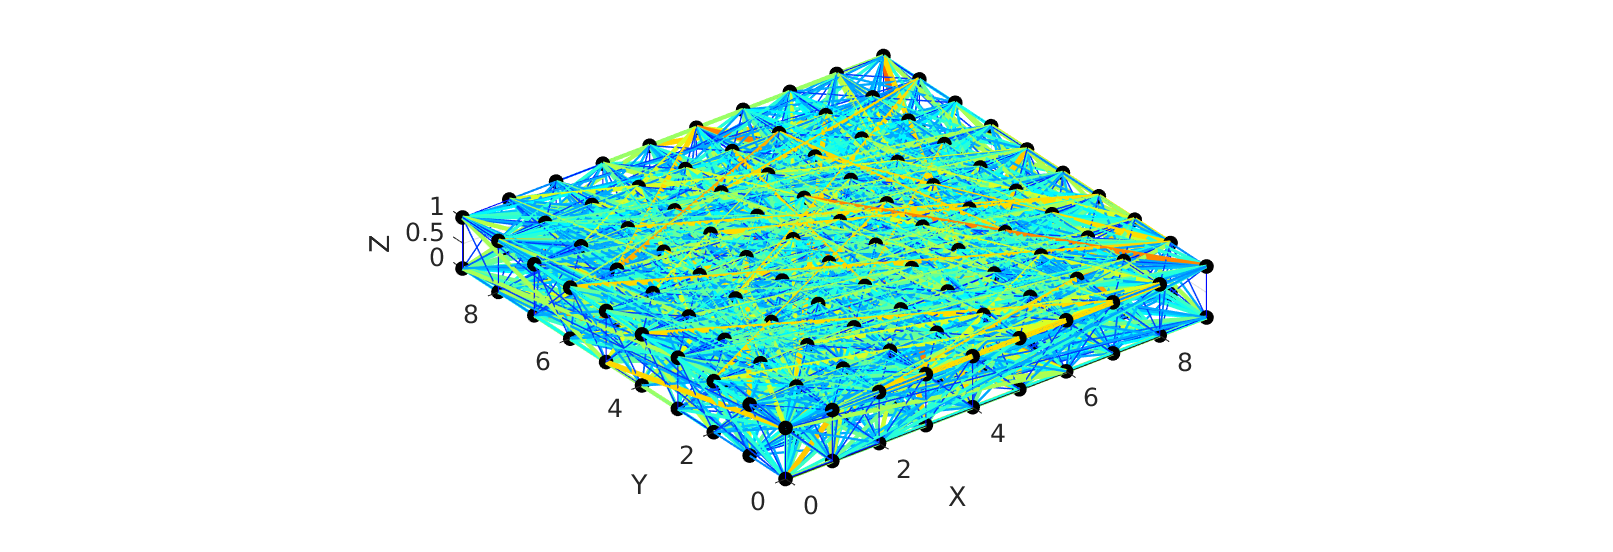
\includegraphics[width=\textwidth]{fig/Sheet_Structure_A}}
 \subfloat[][]{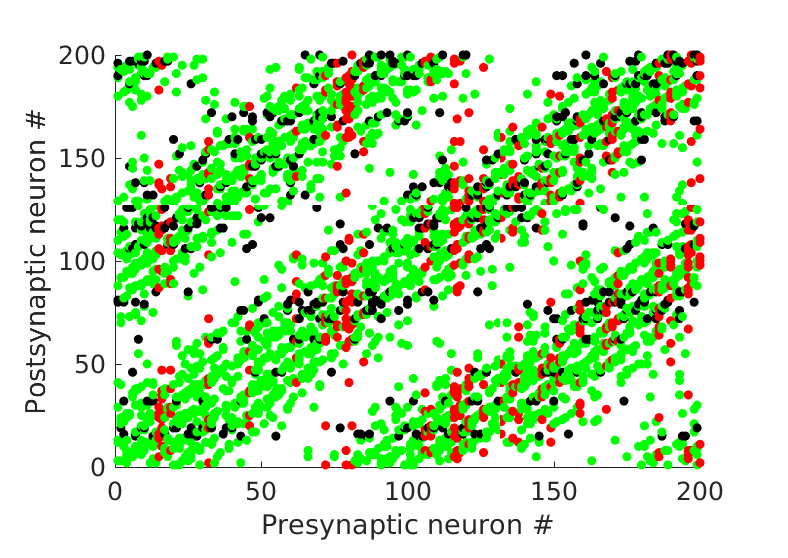
\includegraphics[width=0.4\textwidth]{fig/Sheet_Structure_B}}
 \subfloat[][]{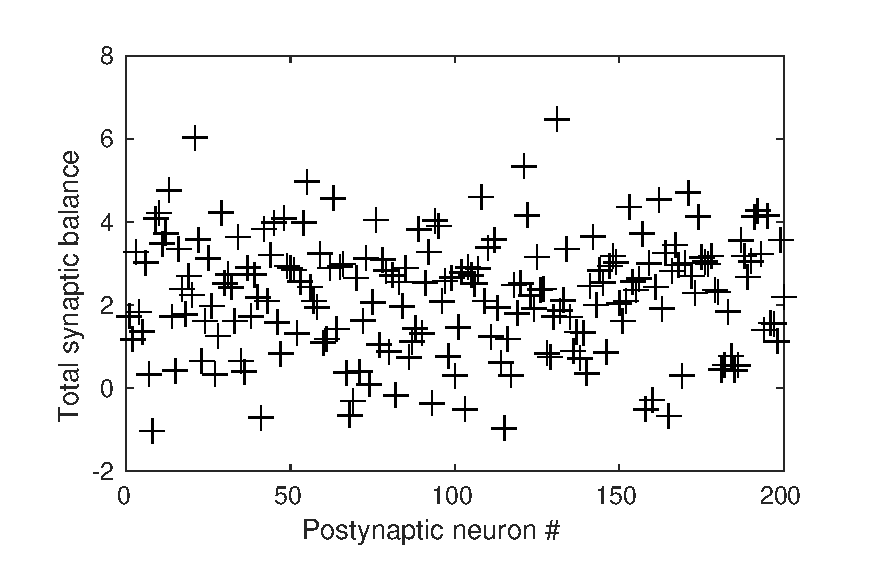
\includegraphics[width=0.4\textwidth]{fig/Sheet_Structure_C}}
\end{figure}

The topology of our sheet combined with our local connectivity rule (eq. \ref{eq:connectivity}) defines the connection distribution of the sheet.
The distribution of post-synaptic connections and delay times are shown in Figure \ref{fig:connection_delay_distrbution_2D} for an example quasi 2-D sheet.
Compared the to minicolumn connection distribution in figure \ref{fig:connection_delay_distrbution} the neurons in our sheet have on average about twice as many connections.
The length of the connections between neurons tends to be longer in the sheet, resulting in a distribution of longer delays 
in figure \ref{fig:connection_delay_distrbution_2D} when compared to figure \ref{fig:connection_delay_distrbution}.
\begin{figure}[!htb]
 \caption{Distribution of (a) number of post-synaptic connections per neuron and (b) delay time. 
          Data was taken from an X=100, Y=100, Z=2 sheet with $\lambda=2.5$, $\kappa=1$ and periodic boundary conditions.  } 
     \subfloat[][]{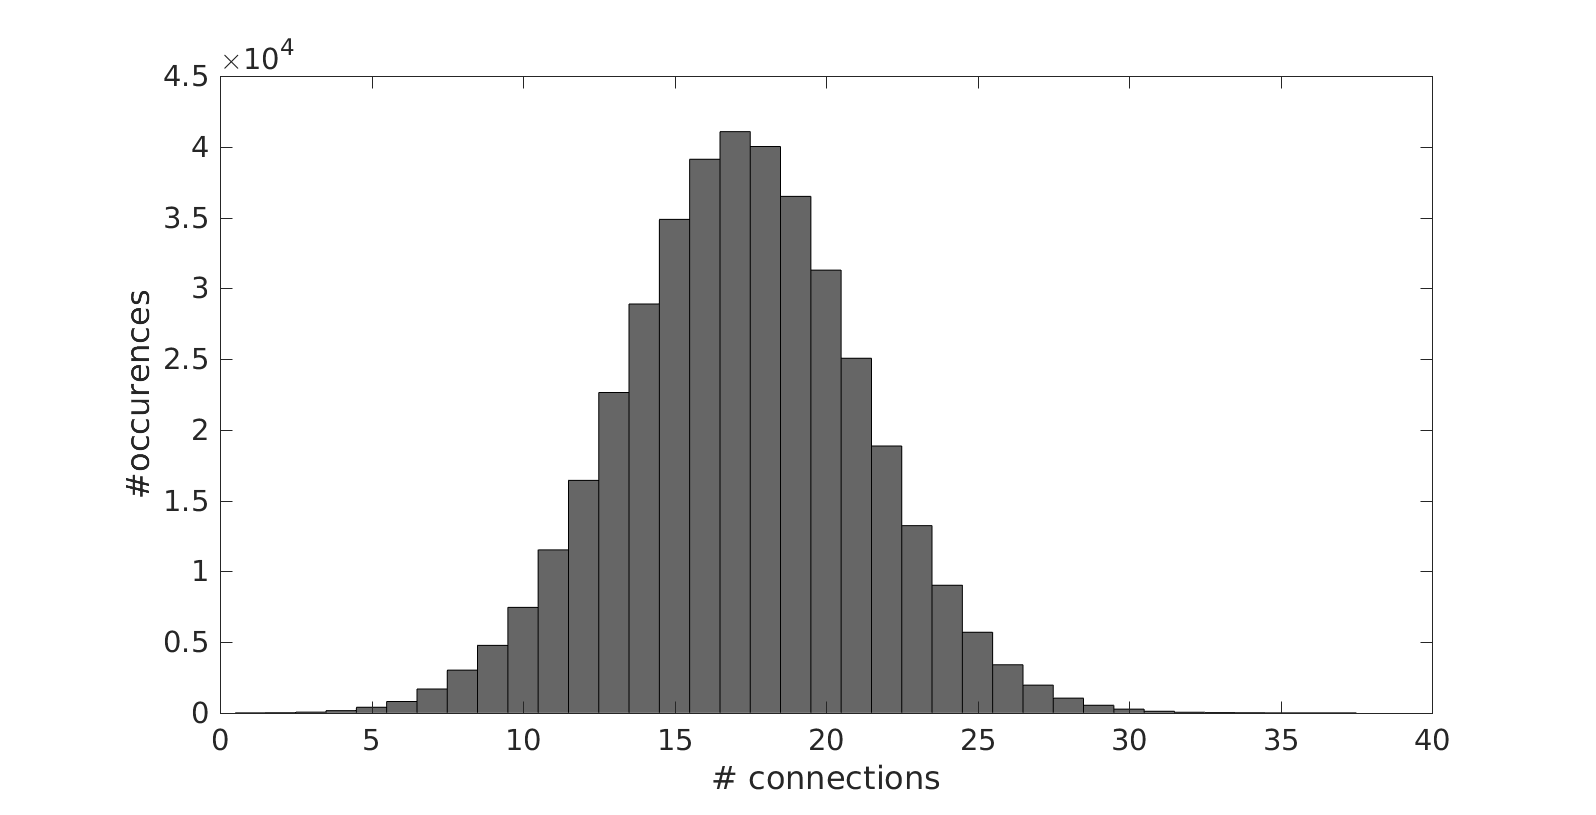
\includegraphics[width=0.6\textwidth]{fig/ConnectionNumberDistribution2D} }
     \subfloat[][]{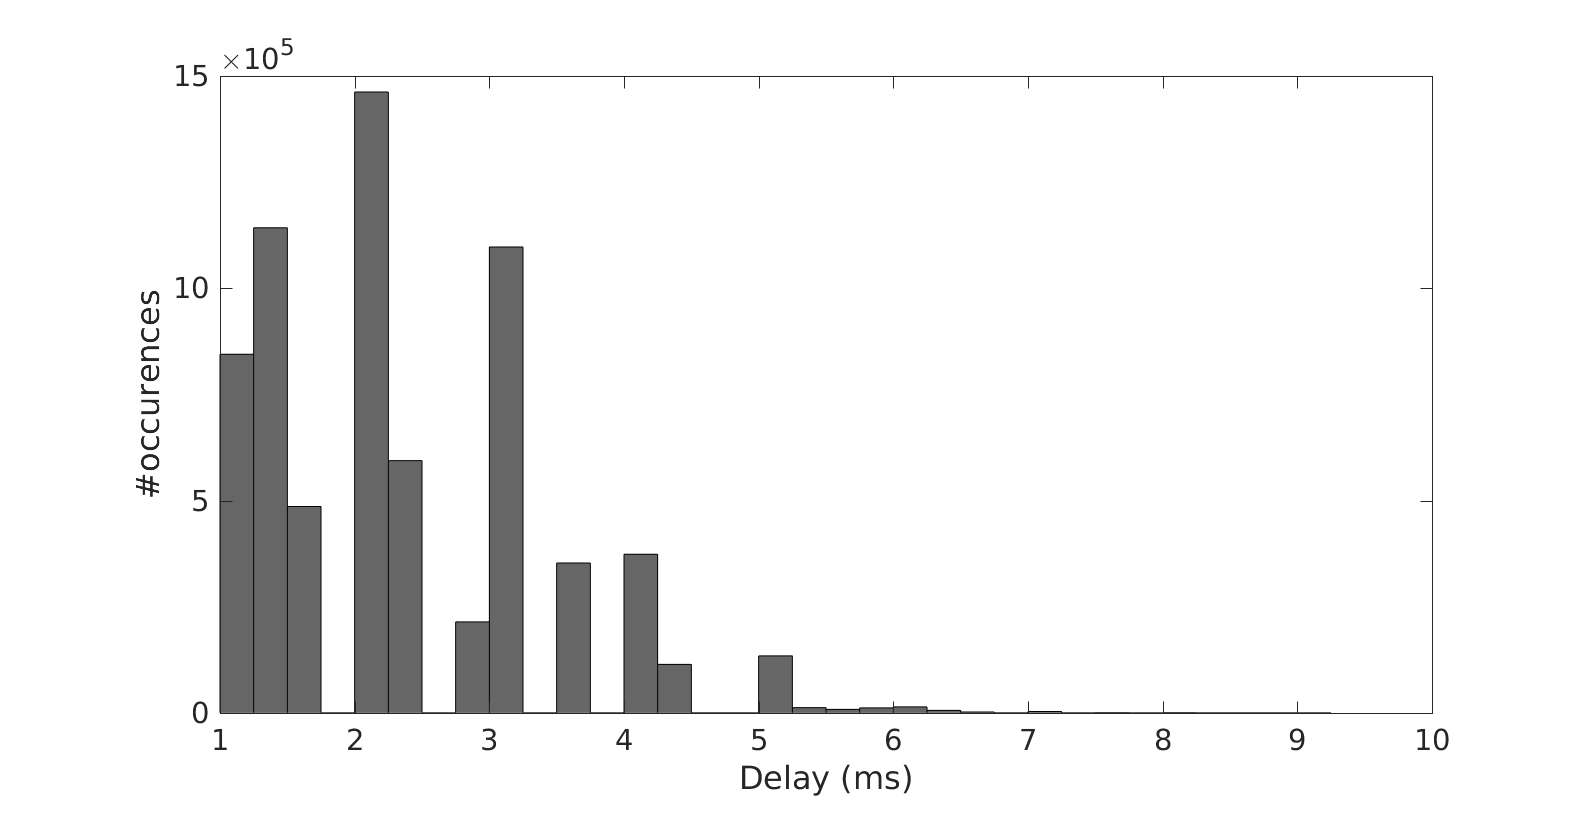
\includegraphics[width=0.6\textwidth]{fig/DelayDistribution2D} }
 \label{fig:connection_delay_distrbution_2D}
\end{figure}
 \FloatBarrier

As we did with our quasi 1-D minicolumn, we first create a purely 2-D sheet of neurons with X=100, Y=100 and Z=1.
Model parameters are fixed at $\Sigma$.
We do not observe traveling waves or other spatiotemporal patterns in this system (Figure \ref{fig:Pure2DRasters_NoWaves}).
\begin{figure}[!htb]
 \caption{ Raster plots from our purely 2-D system do not show coherent spatiotemporal patterns.}
 \label{fig:Pure2DRasters_NoWaves}
 \centering
   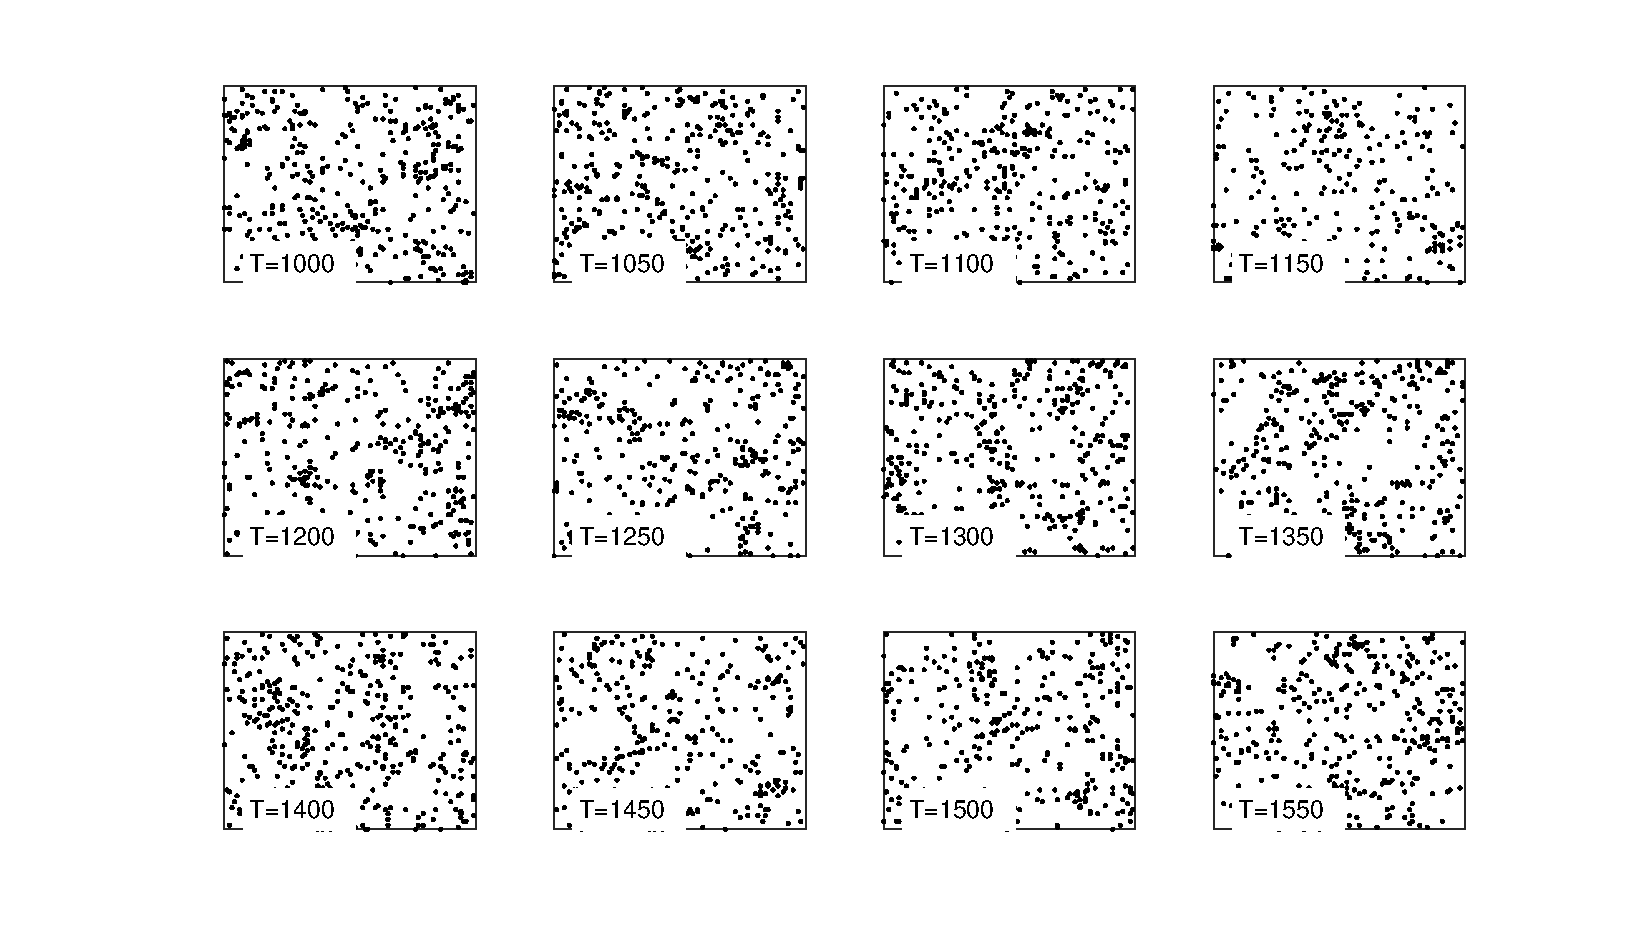
\includegraphics[width=\textwidth]{fig/2DWaveRasters_1LayerNoWaves}
\end{figure}
\FloatBarrier

We then extend our system to a quasi 2-D sheet with X=100, Y=100 and Z=2.
We now observe traveling wave patterns in the system.
These patterns emerge in spite of the high variability in the neuron types, neuron dynamics and connectivity present in our model.
We can clearly see an example of a circular spreading wave emanating from the upper center of figure \ref{fig:2D_waves}.
\begin{figure}[!htb]
 \caption{ Raster plots from our quasi 2-D system with two layers show wave patterns that spread across the surface of the sheet.}
 \label{fig:2D_waves}
 \centering
   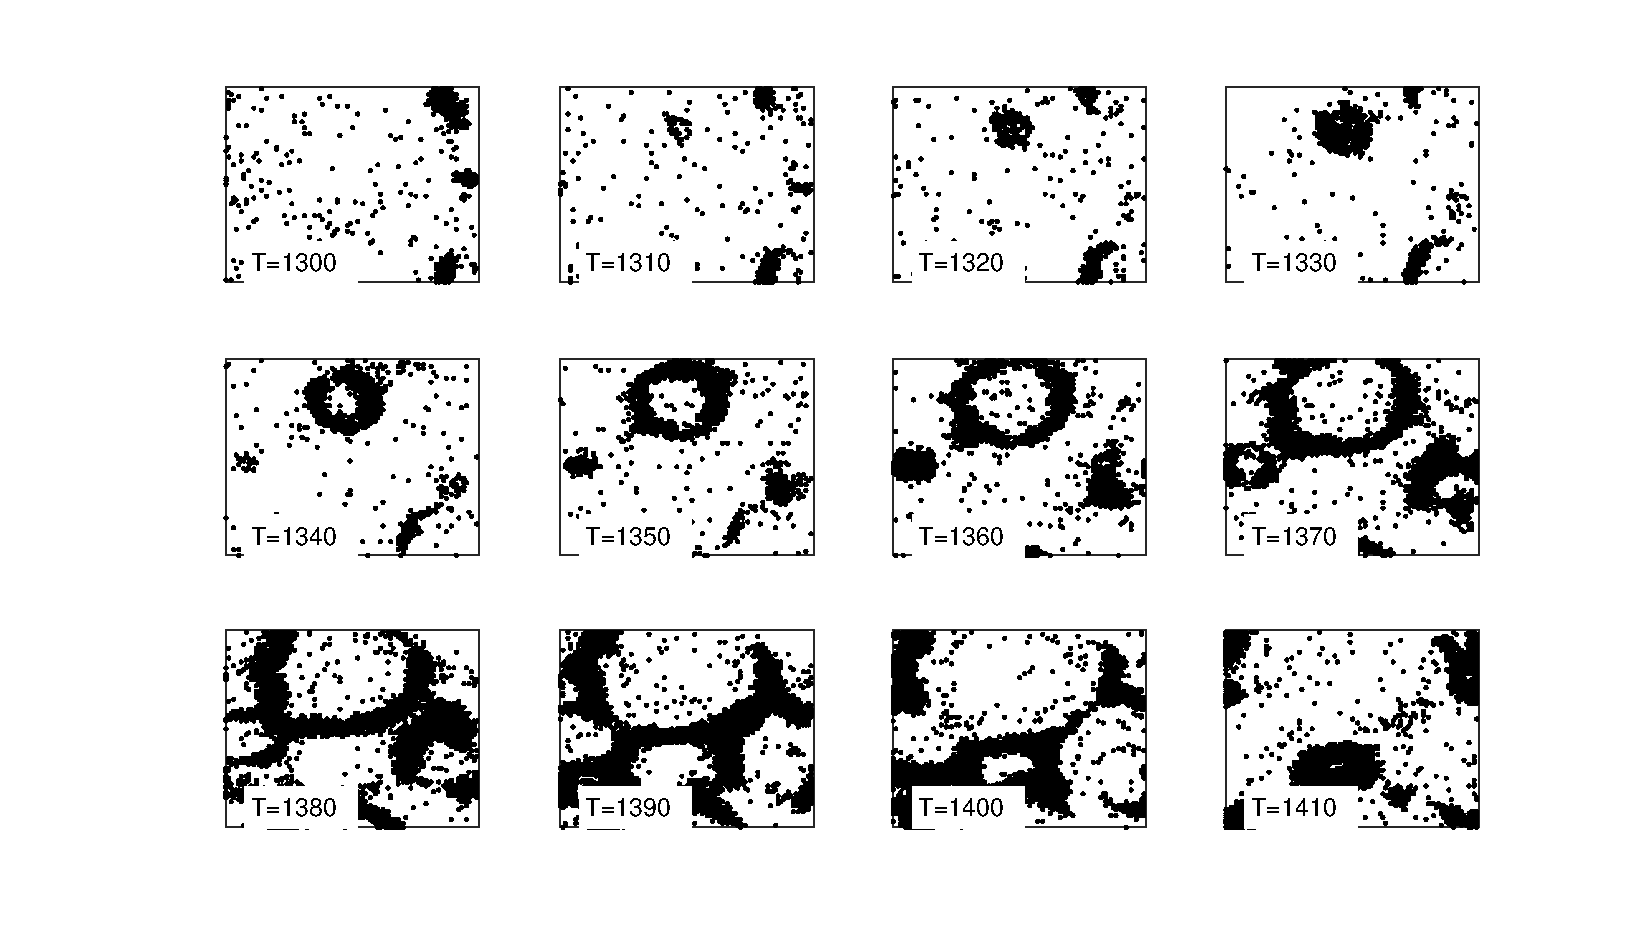
\includegraphics[width=\textwidth]{fig/2DWaveRasters}
\end{figure}

In some simulations we see the formation of large-scale plane waves across the entire system as seen by \citet{keane2015}.
In their work, plane waves were formed when excitation dominated their neuronal system.
The formation of these plane waves in our system does not seem deterministic, as a different random draw of the uniform background stimulus for the same neuronal system may not exhibit plane waves.
Nonetheless, these results show that plane waves can emerge as a stable pattern in systems of this type even when excitation does not dominate.
\begin{figure}[!htb]
 \caption{ Raster plots from our quasi 2.5-D system showing large-scale plane waves moving from top to bottom.}
 \label{fig:2D_plane_wave}
 \centering
   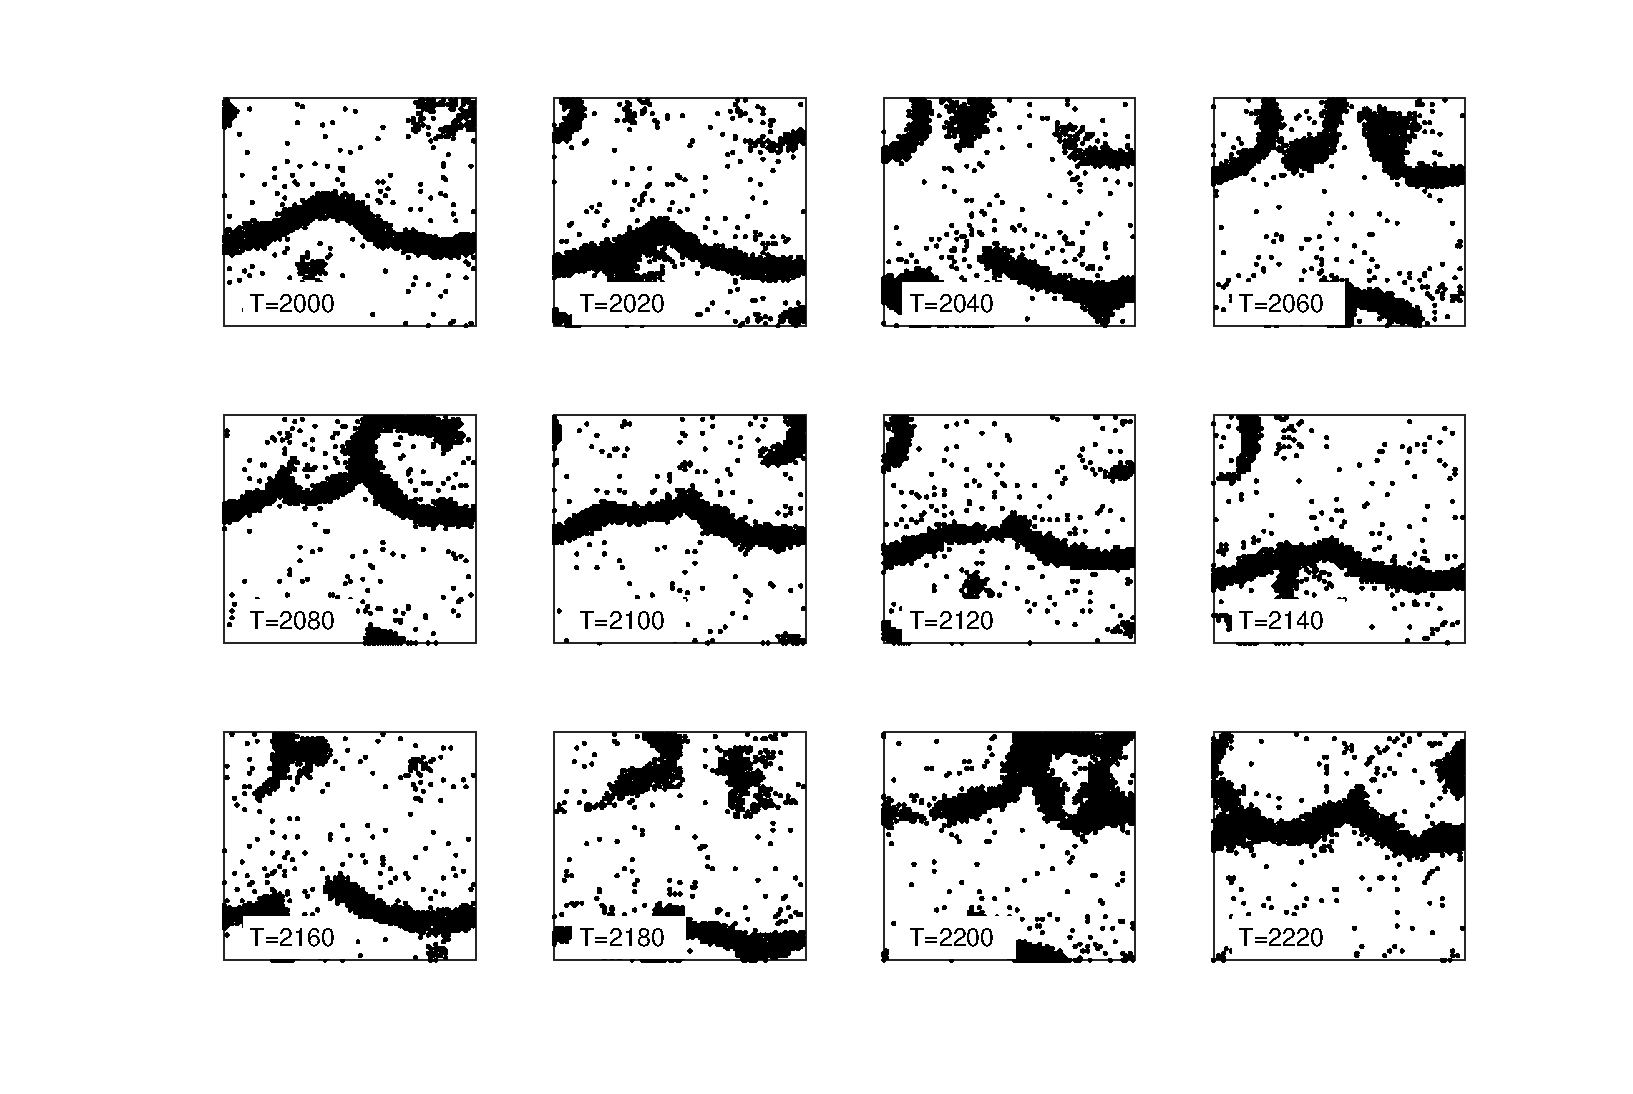
\includegraphics[width=\textwidth]{fig/2DWaveRasters_PlaneWave}
\end{figure}
\FloatBarrier

When the wave speed increases we observe attractor states, where waves spawned from a small number of locations come to dominate the firing activity.
In figure \ref{fig:2DWaveRasters_attractor} we see that the waves come to dominate the firing activity.
\begin{figure}[!htb]
 \caption{ Raster plots from our quasi 2-D system showing an attractor forming near X=70,Y=75.}
 \label{fig:2DWaveRasters_attractor}
 \centering
   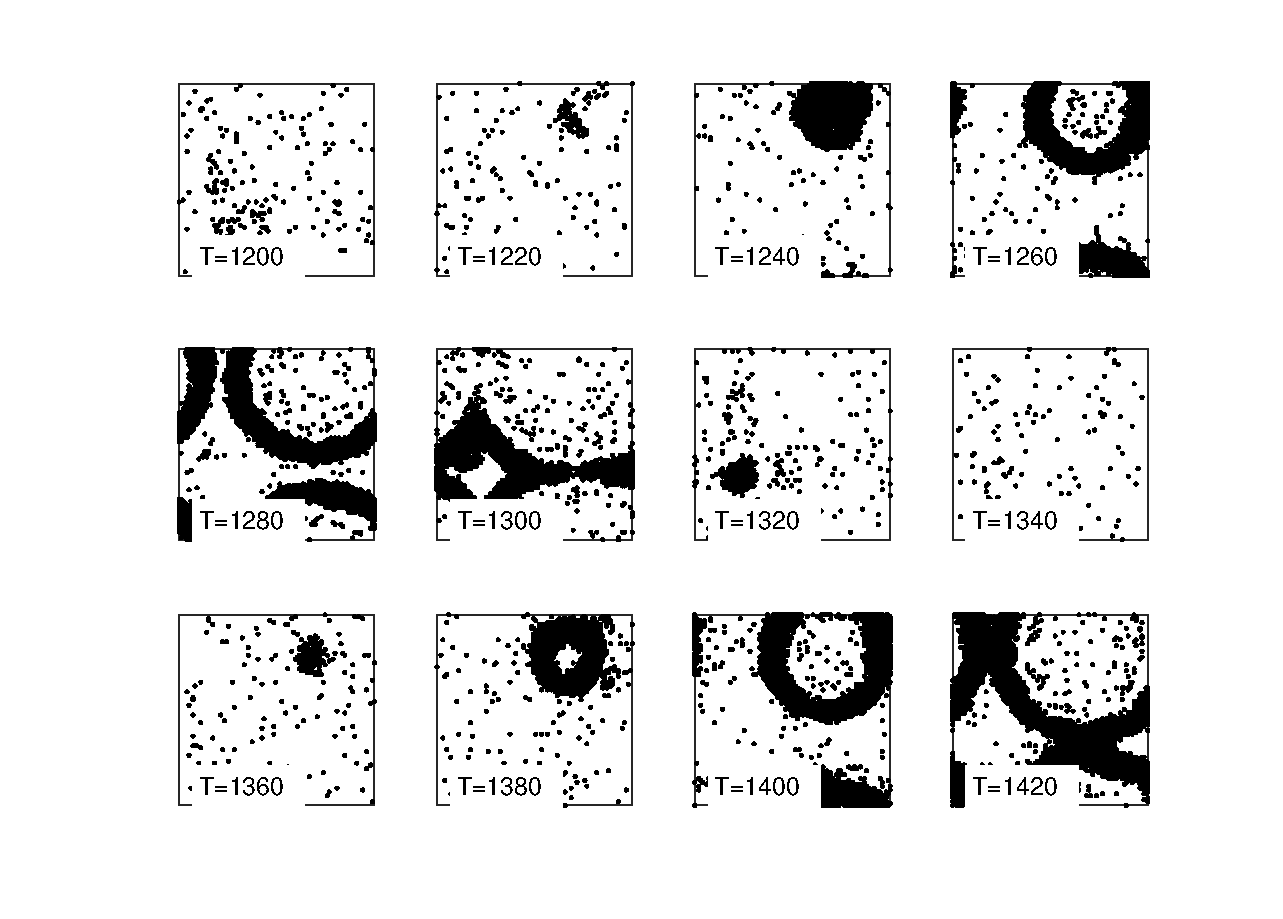
\includegraphics[width=\textwidth]{fig/2DWaveRasters_Attractor_kappa0p1_seed35}
\end{figure}

We suspect that these winner-take-all waves may be spawned by low-threshold spiking inhibitory neurons as seen in our minicolumns (section \ref{sub:wave_initiation}).
To test this hypothesis we plot calculate the density of inhibitory neurons across the sheet using MATlAB's 'ksdensity' function.
\begin{figure}[!htb]
 \caption{ Density plot of inhibitory neurons in the sheet. The color scale covers the top 10\% of the density.
           The area with the highest density of inhibitory neurons includes the location from which the attractor waves are spawned near X=70, Y=75. }
 \label{fig:2DAttractor_InhibDensity}
 \centering
   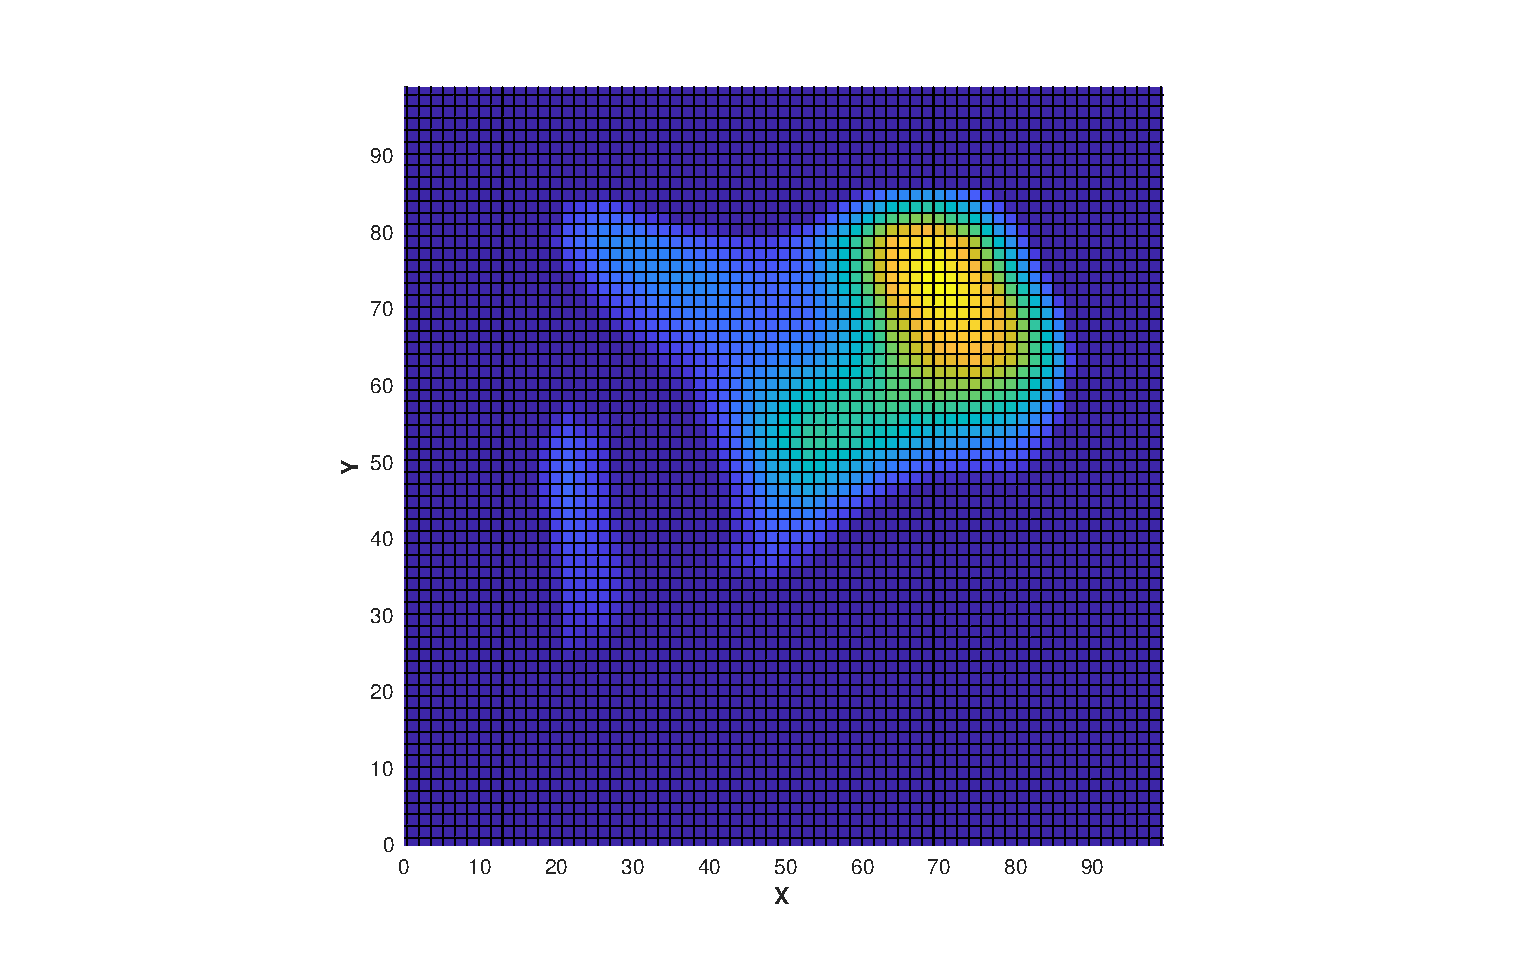
\includegraphics[width=\textwidth]{fig/2DAttractor_seed35_InhibitoryDensity}
\end{figure}

\FloatBarrier

We do not observe spiral waves in our simulations with the model parameters set at $\Sigma$.
With the higher connectivity observed in the sheet (figure \ref{fig:connection_delay_distrbution_2D}) we see circular waves emanating from a point.
Although these waves can combine to form a plane wave structure (figure \ref{fig:2D_plane_wave}), we have not observed spiral wave patterns.
Given that the sheet has higher connectivity than the minicolumn, we reduce the connection strength K from $K=10$ to $K=6$.
The waves at the lower connection strength are thinner and sparser.
We now observe the formation of spiral wave pattern in figure \ref{fig:2DWaveRasters_Spiral}.
\begin{figure}[!htb]
 \caption{ Raster plots showing spiral wave behavior, especially in the center left. The sheet is 200x200x2, $K=6$, $\kappa=0.4$ }
 \label{fig:2DWaveRasters_Spiral}
 \centering
   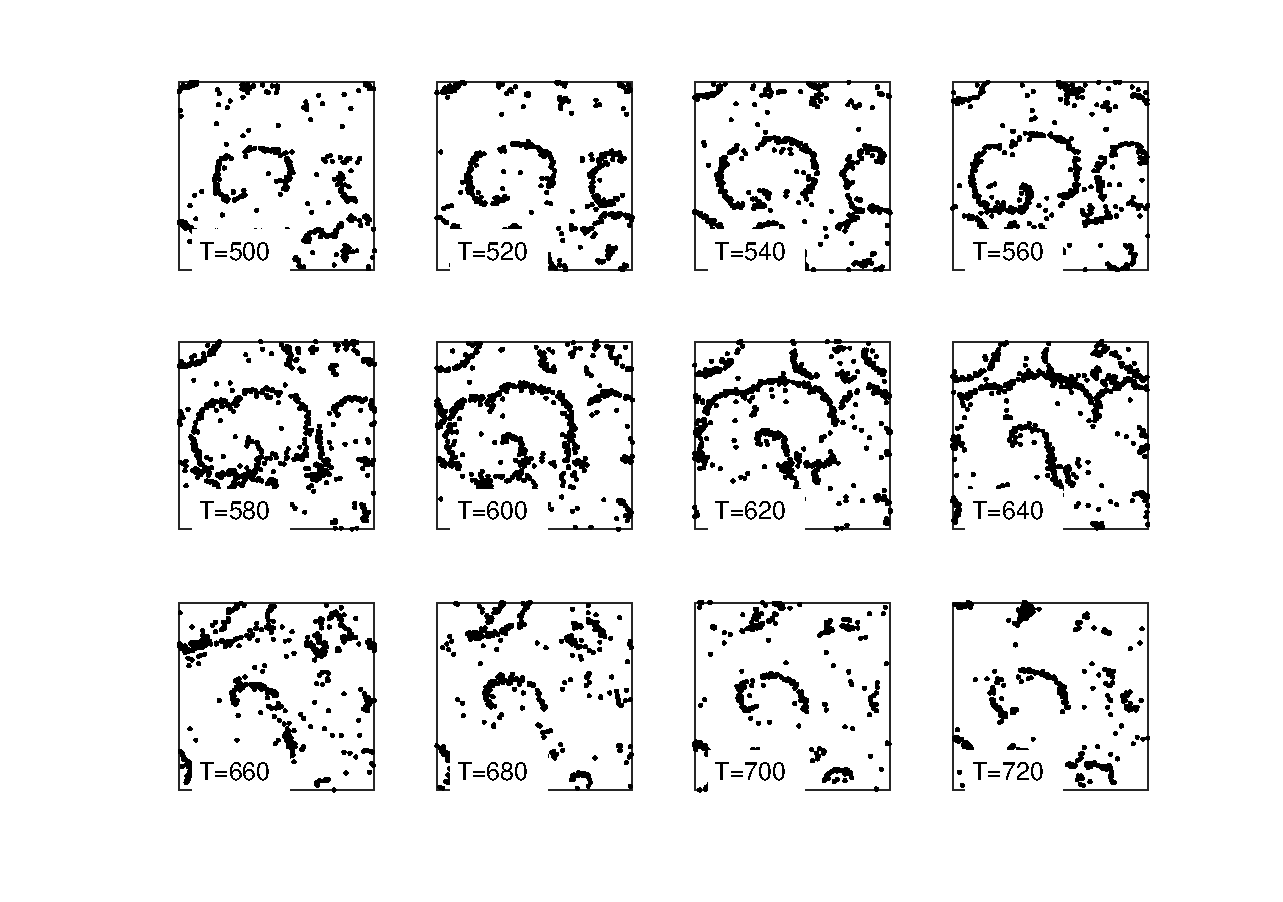
\includegraphics[width=\textwidth]{fig/2DWaveRasters_SpiralWave}
\end{figure}
\FloatBarrier

In \citet{keane2015} traveling waves in 2-D sheets were proposed to explain simultaneous spike timing irregularity with fluctuations in the average firing rate of the ensemble. 
Despite the complex spatiotemporal patterns the overall mean voltage shows a small, steady oscillation.
\begin{figure}[!htb]
 \caption{ After initial fluctuations settle out, the system mean voltage settles into small oscillations.}
 \label{fig:2D_mean_voltage}
 \centering
   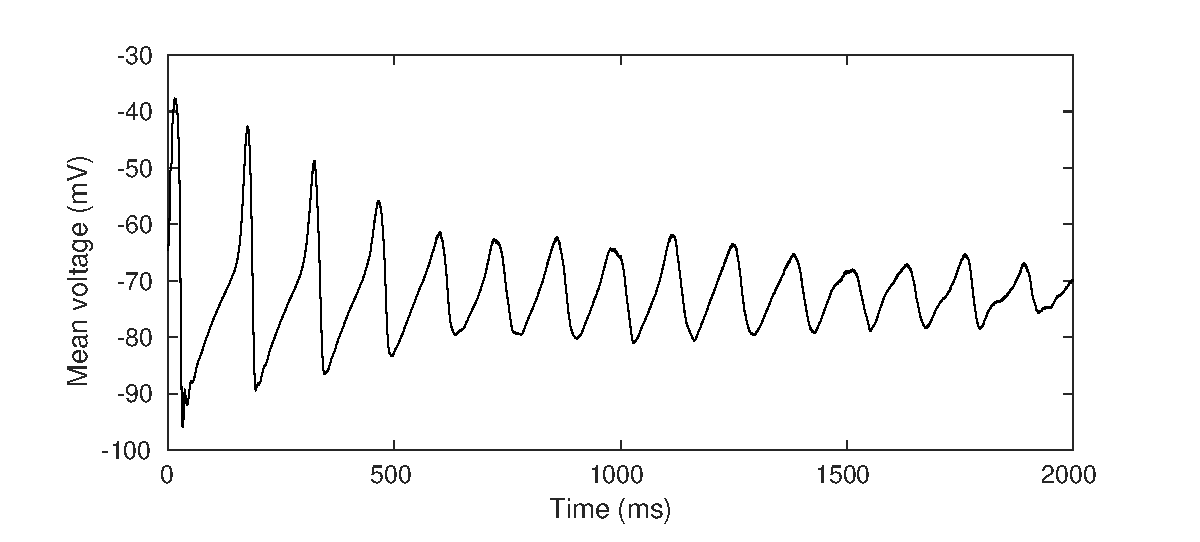
\includegraphics[width=\textwidth]{fig/MeanVoltage_PBC}
\end{figure}

\FloatBarrier

\section{Forests of minicolumns}
Our forest of minicolumns is an ensemble of 400 or 600 minicolumns arranged in a 20x20 or 30x30 pattern.
Each minicolumn is 2x2x10.
A small example foresst is shown in Figure \ref{fig:forest_structure}.
\begin{figure}[!htb]
 \caption{ Example forest of 16 minicolumns arranged in a 4x4 grid, with $1\lambda$ spacing between the closest neurons of any two minicolumns. 
              Each minicolumn has dimensions X=2, Y=2, Z=5, $\lambda$=2.5, and C=0.5. 
          a)  Sheet showing connections between neurons as lines colored using a color scale that indicates the connection length. 
          b)  Connection matrix. E-E connections are green, E-I are black and both I-E and I-I  are red. }
 \label{fig:forest_structure}
 \subfloat[][]{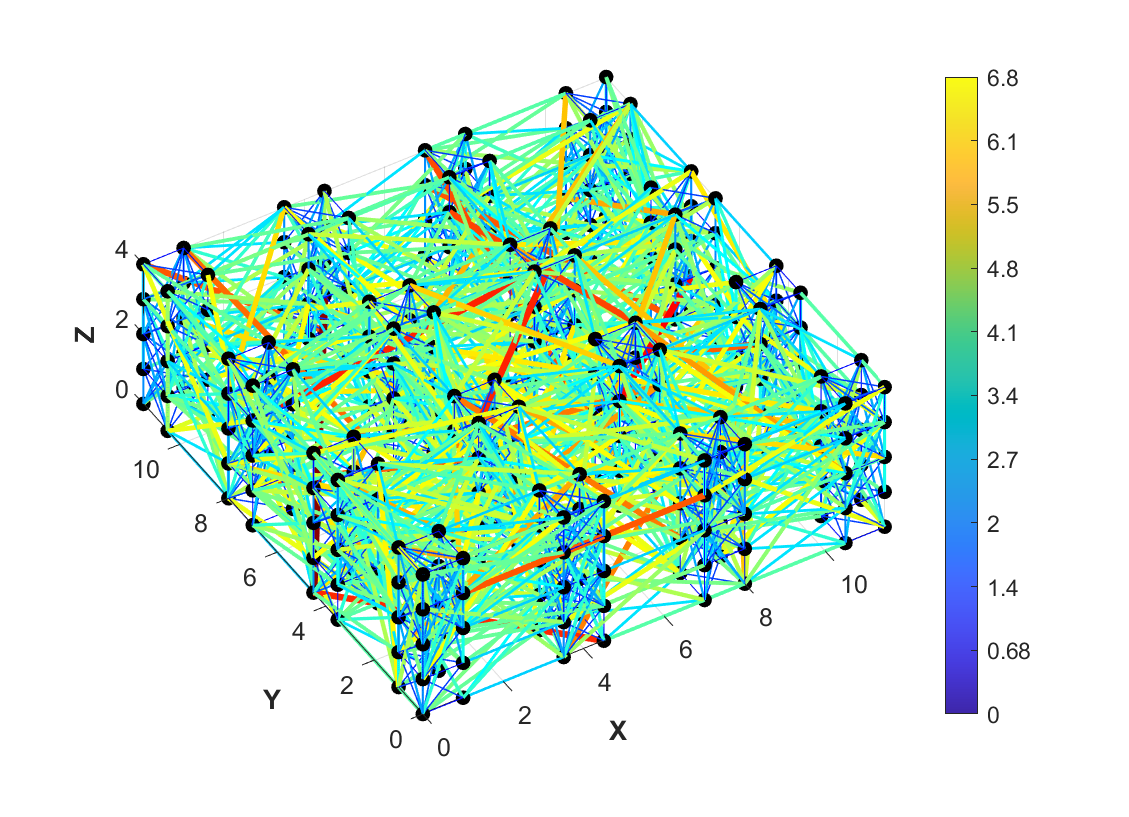
\includegraphics[width=0.75\textwidth]{fig/Forest_Structure_A}}
 \subfloat[][]{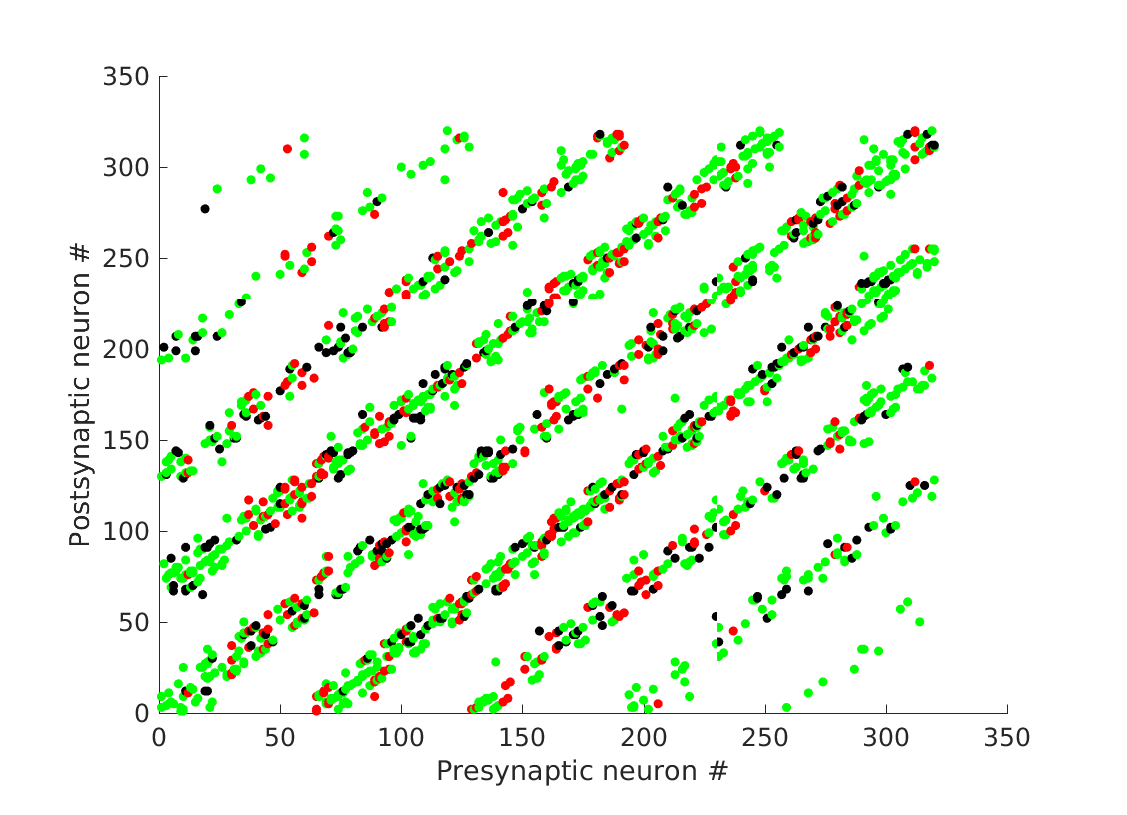
\includegraphics[width=0.75\textwidth]{fig/Forest_Structure_B}}
\end{figure}
\FloatBarrier

We wish to compare the overall 
The distribution of post-synaptic connections and delay times are shown in Figure \ref{fig:connection_delay_distrbution_forest} for an example minicolumn.
\begin{figure}[!htb]
 \caption{Distribution of (a) number of post-synaptic connections per neuron and (b) delay time. Data was taken from a 20x20 forest of 400 minicolumns, each minicolumn 2x2x10, $\lambda=2.5$, $\kappa=1$.  } 
     \subfloat[][]{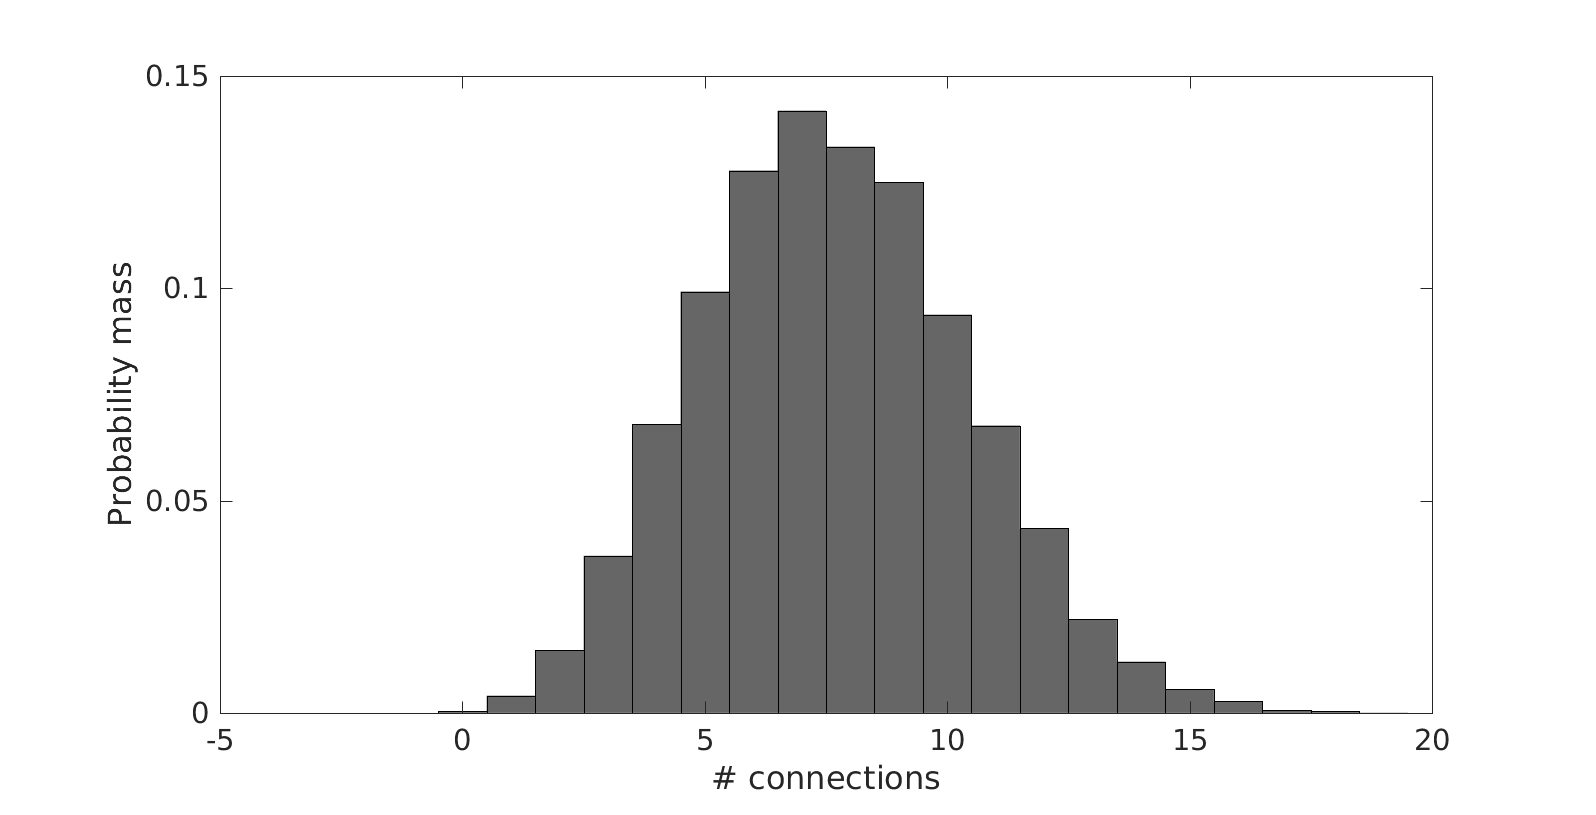
\includegraphics[width=0.6\textwidth]{fig/ConnectionNumberDistributionForest} }
     \subfloat[][]{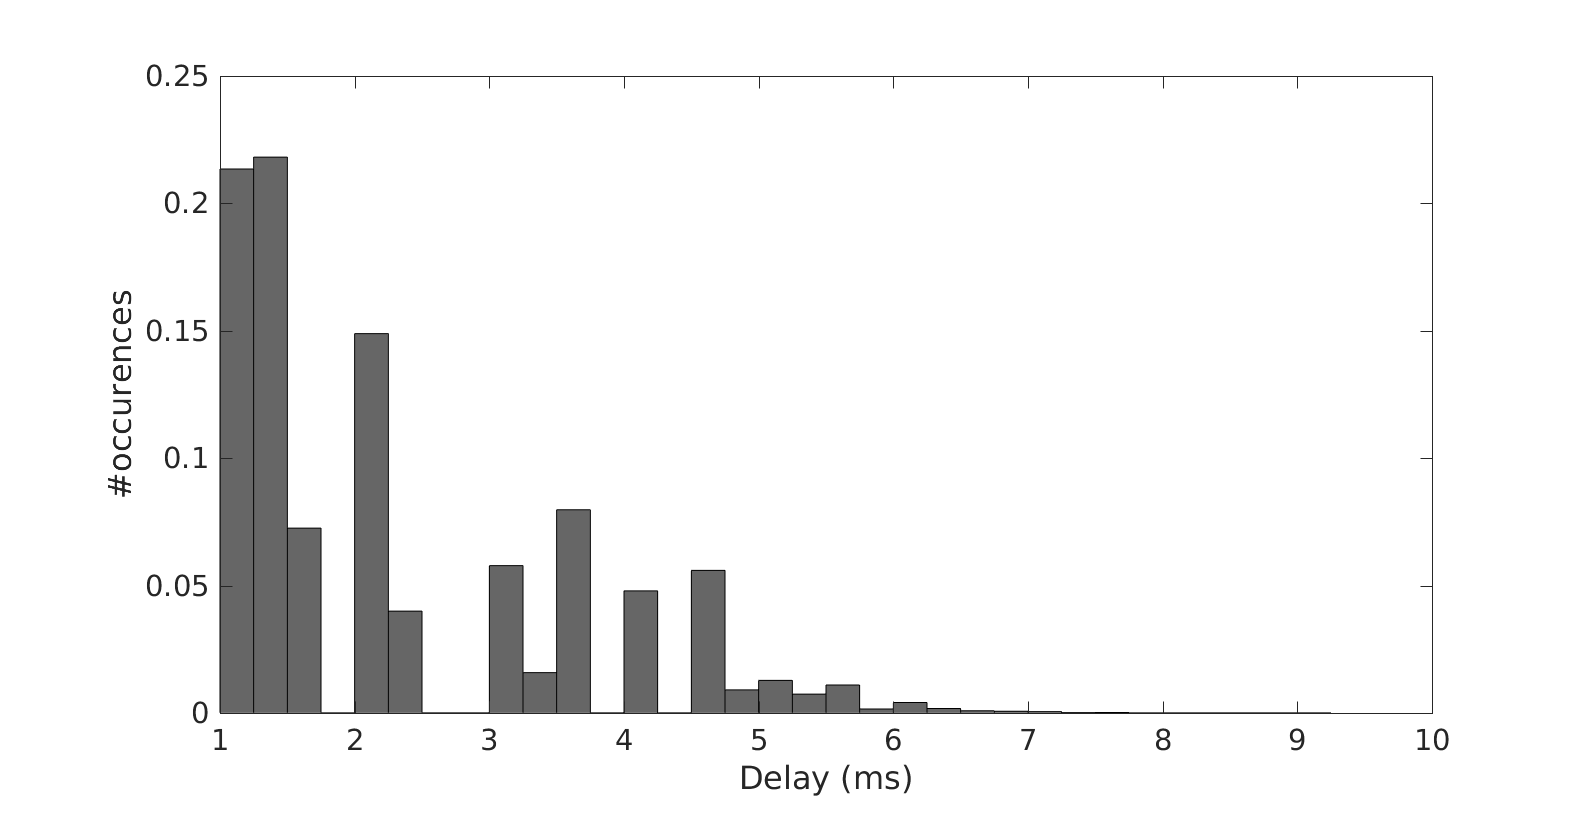
\includegraphics[width=0.6\textwidth]{fig/DelayDistributionForest} }
 \label{fig:connection_delay_distrbution_forest}
\end{figure}
 \FloatBarrier

We stimulate the forest with a uniform background stimulus. 
With $M=5$ there are many competing waves resulting in small-scale waves with many collisions.
We decrease M to 2 and increase K from 10 to 14.
We then observe traveling wave patterns in the forest.
\begin{figure}[!htb]
 \caption{ Raster plots from a forest of minicolumns with uniform background stimulus.}
   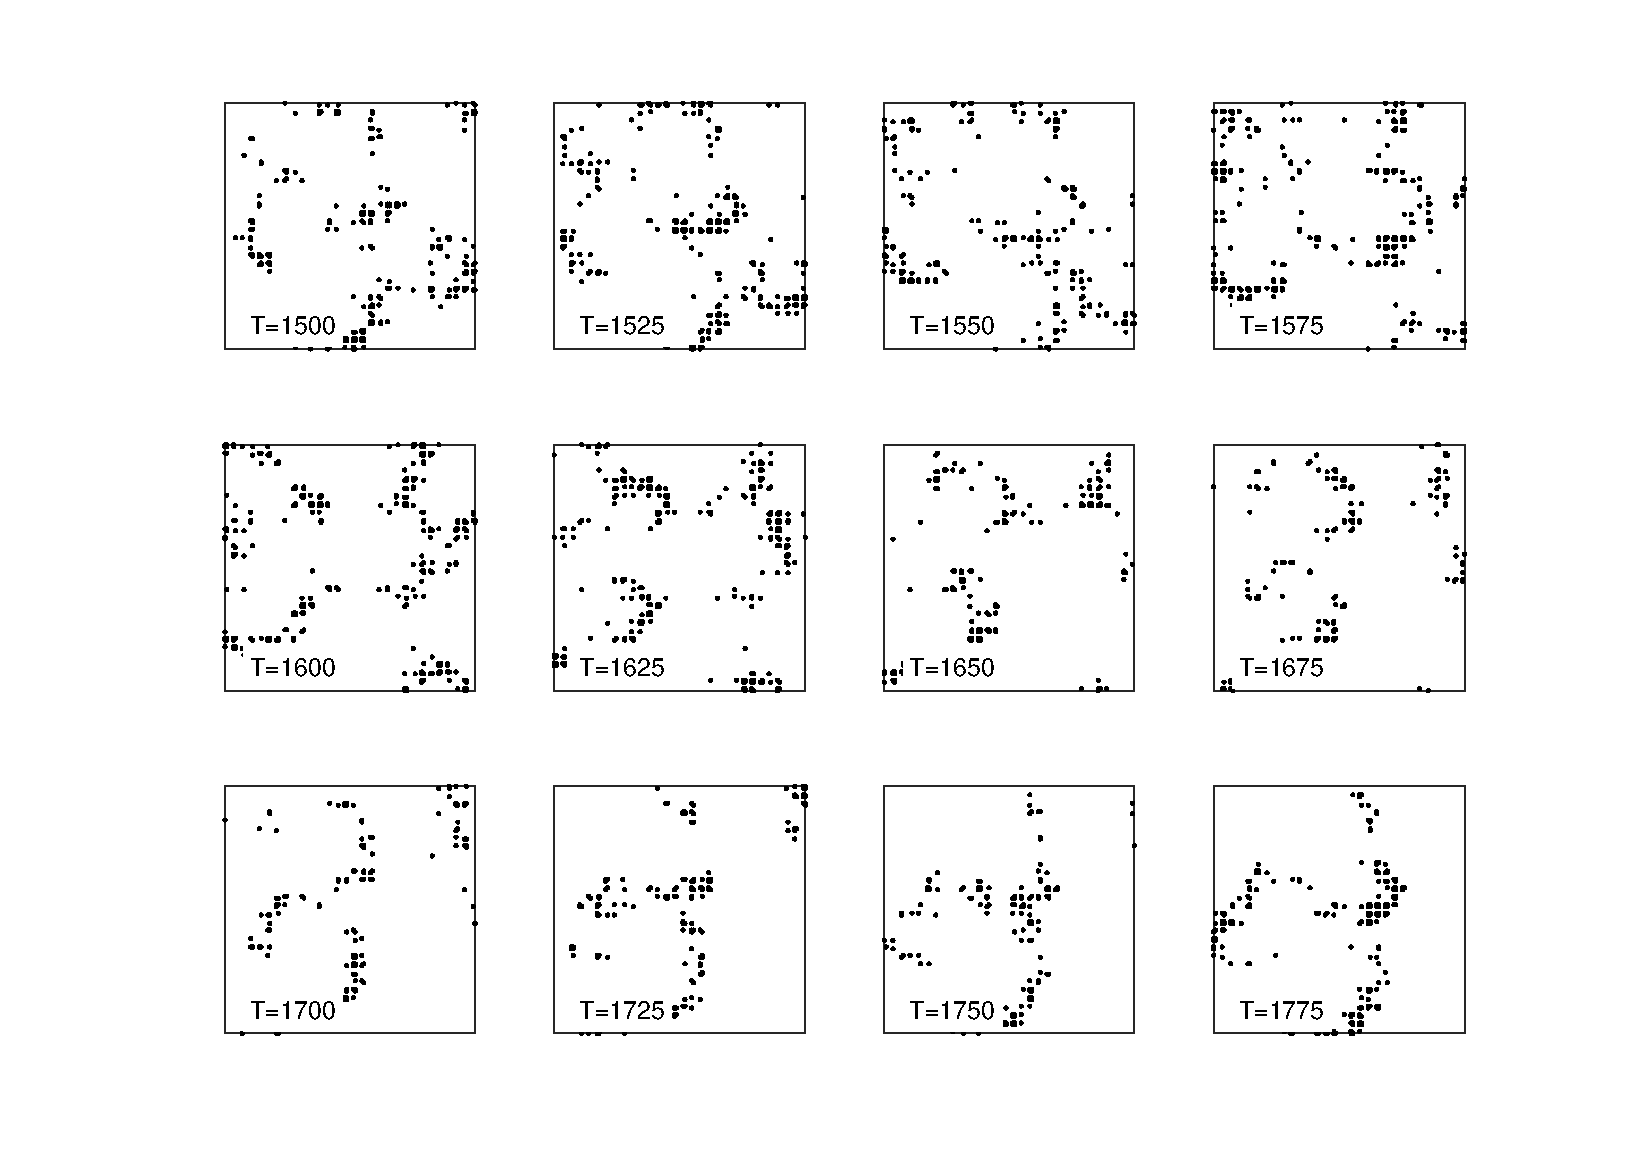
\includegraphics[width=\textwidth]{fig/ForestWaveRaster_Background_K14_M2}
   \label{fig:ForestBackground}
\end{figure}

We perform individual wave trials as in section \ref{sub:propagation_speed}.
In this case stimulate the minicolumn at X={0,1}. Y={0,1}.
We stimulate the first two layers Z={1,2}.
We observe a single wave traversing the forest in Figure \ref{fig:2_5D_Wave}.
\begin{figure}[!htb]
 \caption{ Raster plots from a forest of minicolumns looking down on the X/Y plane. 
           The 2x2 minicolumn in the lower left corner was stimulated at time $t=10\ ms$.}
   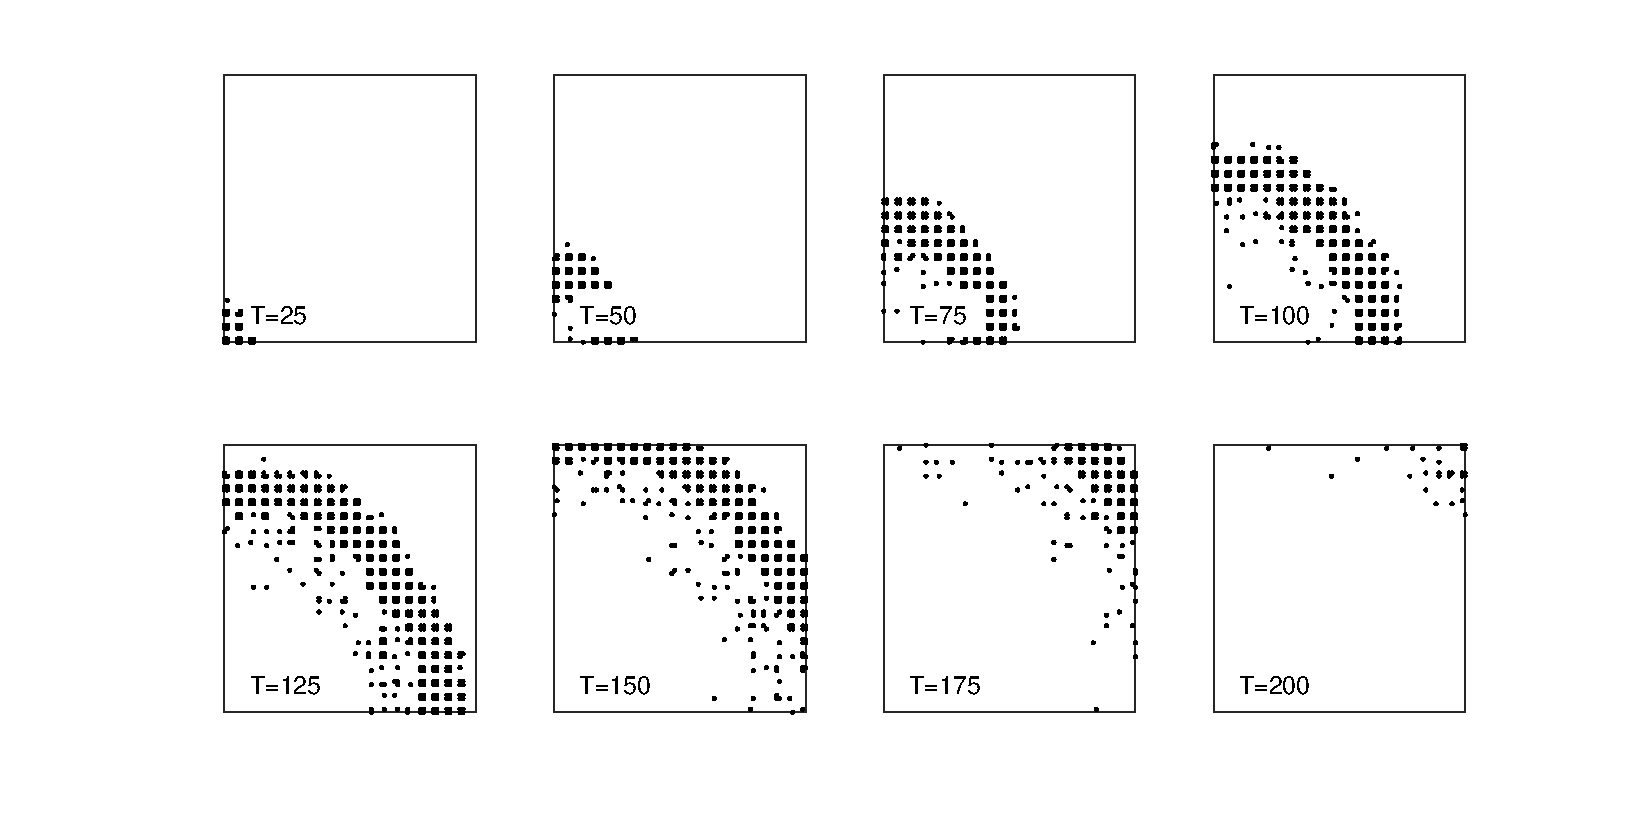
\includegraphics[width=\textwidth]{fig/Rasters_2_5D_Wave}
   \label{fig:2_5D_Wave}
\end{figure}


\FloatBarrier


\endinput
%%
%% End of file `example-1.tex'.
